\justifying
\section{Introduction}
The thermomechanical and electrical properties of low dimensional carbon nanomaterials make them candidates for the next-generation conductive light-weight high-strength architectures.\cite{Park2009,Liu2011,DeVolder2013,Cong2014} However, the cost and difficulty associated with scalable synthesis of macroscopic architectures from low dimensional carbon materials\cite{DeVolder2013,Cong2014} leaves room for improvement.

Recent work on graphene oxide (GO) indicates there is potential for nanomanufacturing via cost-effective solution techniques\cite{Cong2014,Aboutalebi2011,Kumar2014,Zheng2013,Jia2014} that retain GO properties\cite{Dikin2007,Dreyer2010,Liu2012} such as thermal conductivity,\cite{Balandin2011} mechanical stiffness,\cite{Lee2008} elasticity,\cite{Gomez2008} and optical transparency.\cite{Kim2009} Moreover, the GO oxygen functional groups act as both a spacer,\cite{Dikin2007,Sun2013,Han2013,Smith2014,Joshi2014} and a functionalized site for molecular adsorption,\cite{Stankovich2006,Mkhoyan2009} which enables GO conversion into nanomorphologies that could be used for applications such as filtration membranes,\cite{Han2013} supercapacitors,\cite{Zhang2010} electrochemical sensors,\cite{Shao2012} and hydrogen storage devices.\cite{Zou2010} One potential nanomorphology is a GO nano-scroll (GONS) \textit{i.e.}, a GO sheet rolled into a spiral-wound structure (Fig.~\ref{fig1}a). GONS are similar in morphology to a carbon nanotube (CNT), but with a significantly more accessible inter-wall area.

Previous work on the formation of spiral-wound graphene-based structures has focused on graphene nanoscrolls (GNS). Studies have demonstrated that there is an energy barrier (100s to 1000s J mol$^{-1}$) to initiate GNS formation after which the scrolling process self-propagates due to $\pi - \pi$ interactions forming a nanoscroll with an internal diameter of $\approx2$ nm.\cite{Braga2004,Chen2013,Patra2009,Kim2010} The two primary methods to overcome the scrolling energy barrier are: i) template initiators such as carbon nanotubes,\cite{Kim2010,Zhang2010,Xia2010,Perim2013,Wang2015,Calvaresi2013} nanodroplets,\cite{Calvaresi2013,Patra2009} and nanoparticles;\cite{Wang2012,Sharifi2013,Zhao2014,Zhao2014a} and ii) external stimuli such as ultrasonication,\cite{Wang2012,Calvaresi2013,Viculis2003,Roy2008} microwave sparks,\cite{Zheng2011} mechanical manipulation,\cite{Chen2013,Li2005,Gao2010,Li2013} thermal processing,\cite{Wang2015,Zhao2014,Zhao2014a} electric fields,\cite{Sidorov2009} and solvents.\cite{Savoskin2007,Xie2009} GNS have diameters of $\approx 20 - 600$ nm,\cite{Li2005,Savoskin2007,Roy2008,Zhao2014,Kim2010,Zheng2011,Wang2012} lengths of $\approx 0.7 - 10\ \mu$m,\cite{Li2005,Savoskin2007,Kim2010,Zheng2011,Wang2012} and the dimensions are a function of experimental processing conditions and graphene flake surface chemistry.

In contrast to GNS, studies on GONS have been relatively limited. For example, previously synthesized GONS cannot be characterized by metrics such as dimension since the structures are typically composed of crumpled and/or folded GO\cite{Li2013,Fan2015} instead of a properly scrolled morphology. GONS have been synthesized by mechanical manipulation\cite{Li2013,Fan2015} and/or chemical initiators.\cite{Gong2014,Rani2015} In contrast, GONS formation via ultrasonic irradiation has not been investigated in depth. Ultrasonic pressure waves results in transient bubble cavitation, \textit{i.e.}, the sequential nucleation, growth, and collapse of microscopic bubbles.\cite{Patil2007} The ultrasonic energy imparted to bubbles and, in turn the GO flakes, provides the scrolling activation energy to form GONS. However, such extreme energy release (bubble vapor $T \approx4000$ K; bubble interface $T \approx800$ K) will also chemically modify and cleave the GO flakes impacting the surface chemistry and morphology of the resulting GO nano-structures.\cite{Goncalves2014}

Here, we complete a systematic study on the effect of ultrasonic frequency, power density, and irradiation time on GONS production, morphology, dimensions and surface chemistry. GO was synthesized via the oxidation of graphite flakes following a modified Hummers' method.\cite{Hummers1958,Perrozzi2015} The GO was subjected to two frequencies of ultrasonic irradiation; 20 kHz low frequency (LF) irradiation generated by a commercial tip-sonicator and 390 kHz high frequency (HF) irradiation generated by a homemade reactor, at both low and high power densities (Fig.~\ref{fig1}b). The time-dependent structure and morphology of the GO and GONS was analyzed by scanning (SEM) and transmission (TEM) electron microscopy, and the GO and GONS surface chemistry and interlayer interactions were analyzed by Raman spectroscopy and X-ray photoelectron spectroscopy (XPS).

\begin{figure}[t!]
  \centering
  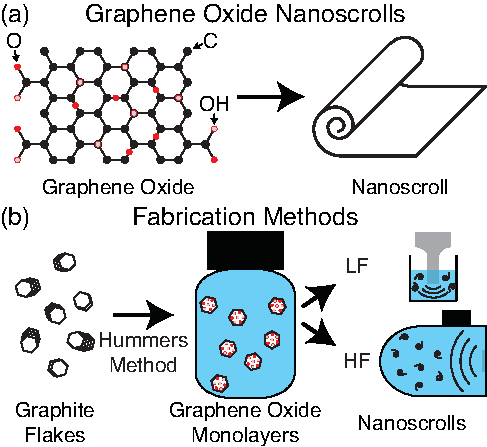
\includegraphics{paper1/Fig1.pdf}
  \caption{\textbf{Structure and fabrication methods of GO and GONS.} \textbf{(a)} Illustration of the GO flake chemistry showing the arrangement of the oxygen functional groups, and the cross-sectional morphology of GONS. \textbf{(b)} Summary of the GONS fabrication process starting from graphite flakes and demonstrating the difference between the low frequency (LF) and high frequency (HF) processing.}
  \label{fig1}
\end{figure}


\section{Methods}

\subsection{Graphene Oxide Synthesis}

The GO solution was prepared using a modified Hummers' method\cite{Hummers1958} with additional pre-processing of the graphite powder.\cite{Kovtyukhova1999} Additional details can be found in Appendix B.

\subsection{Graphene Oxide Treatment}

For the LF treatment, 8 mL of GO solution was dispersed in 392 mL of ethanol(EtOH) (final GO concentration 0.002 wt\%) in a 600 mL glass beaker, and was subjected to 20 kHz LF tip-sonication treatment (Sonifier S-450D; from \textit{Branson Ultrasonics Corp.} with high gain horn) at 10\% and 90\% of the maximum amplitude ($130\ \mu$m for the used tip geometry), which results in a calorimetric power density (see below) of $\approx10$ W ($9.7 \pm 1.3$ W) at 10\% and 100 W ($99.9 \pm 13.2$ W) at 90\% respectively. To explore the impact of the GO solution volume on the observed GO and GONS morphologies, the LF treatment was also carried out at a reduced volume of 2 mL of GO solution dispersed in 98 mL of EtOH (in a 150 mL glass beaker) at 10\% of the maximum amplitude ($\approx10$ W of power according to calorimetry). For the HF treatment, 25 mL of GO solution was dispersed in 1.175 L of EtOH (final GO concentration 0.002 wt\%) and processed via 390 kHz HF treatment in a reactor comprised of a 1.5 L jacketed glass reactor composed (\textit{Chemglass Inc.}) and a cylindrical PbZr$_{x}$Ti$_{1-x}$O$_{3}$ (PZT) piezoelectric crystal (5 cm diameter, 0.35 cm thickness, PZT-840, APC International, Ltd.). The piezo was attached to a steel plate (12.7 cm diameter, 0.05 cm thick) using a conducting silver epoxy (\textit{CHO-bond 584}, \textit{Parker Chomerics}) with electrical leads connected using a non-lead solder. The electrical signal used to drive the PZT crystal is produced by an arbitrary waveform generator (\textit{Agilent}; 33522A) and was amplified by a linear RF power amplifier (ENI; 2100L; 100 W max; 10 kHz$-12$ MHz). Since there are no commercially available setups capable of ultrasonic treatment at frequencies $\geq 100$ kHz, the HF setup used here was custom built for this experiment. On the other hand, there are large-scale commercial systems on the market that capable of ultrasonic treatment at $20-40$ kHz, e.g. from Industrial Sonomechanics, LLC, and \textit{Branson Ultrasonics Corp.}
The HF power was controlled by setting the arbitrary waveform generator peak-to-peak voltage amplitude, where 0.8 V peak-to-peak was used for HF(1 W) $1.2 \pm 0.2$ W, 1.8 V peak-to-peak for HF(10 W) $10.2 \pm 2.3$ W, and 2.5 V peak-to-peak for HF(20 W) $19.7 \pm 3.8$ W with power determined via calorimetry. The ultrasonically-irradiated GO solution was then drop-cast on either a Si wafer (SEM/Raman/XPS) or a TEM grid for further characterization.
The calorimetric powers ($Q$) were calculated $Q = mC_{\mathrm{p}}\Delta T$ where $C_{\mathrm{p}}$ is the specific heat capacity of ethanol, $m$ is equal to 0.32 kg and 0.95 kg for HF and LF, respectively, and $\Delta T$ is the change in temperature recorded during irradiation time.

\subsection{Structure and Morphology Characterization}

\textbf{Scanning electron microscopy (SEM):} The surface morphology of the GO flakes was characterized using a \textit{Zeiss ULTRA} Field Emission Scanning Electron Microscope with an In-lens secondary electron detector. In order to image the GONS, a working distance of $3 - 4$ mm, an acceleration voltage of $3 - 4$ kV, and an aperture of 20 $\mu$m was utilized. These operating conditions allow visualization of the GONS overlapped structure and recognition of the fine details on the order of tens of nanometers. The statistical SEM image analysis of the GO and GONS was completed using \textit{ImageJ} (see Fig.~\ref{figS7_AppB} in the Appendix B), where $> 300$ GO flakes and $> 15$ GONS were analyzed for each processing time.

\textbf{Transmission electron microscopy (TEM):} The GO structures were analyzed using a {JEOL-2100 LaB6 TEM} (see Fig.~\ref{figS2_AppB} in the Appendix B). The accelerating voltage was 80 or 200 keV depending on the image. The second largest condenser aperture was used. The GO and GONS were drop-cast on a 200 mesh Cu TEM grid covered by a continuous carbon film (\textit{Ted Pella, Inc.}).

\textbf{Raman spectroscopy:} Raman spectra were acquired using a \textit{WITec} Confocal Raman Microscope/SNOM/AFM. The laser wavelength was 532 nm and the spectra are characterized using a 0.3 s integration time of at least 20 spectra. Raman intensity maps (500 acquisition points for a $25 \times 25\ \mu$m image) were constructed by scanning during acquisition. The spectra were deconvoluted using a single Lorentzian and a Breit-Wigner-Fano for the D-and G-band, respectively.

\textbf{Atomic force microscopy (AFM):} The thickness of the GO and GONS was measured with an \textit{Asylum Cypher} AFM using an \textit{Olympus 200TS} cantilever (resonance frequency $\approx 150$ kHz). The images were acquired in amplitude modulation mode\cite{Paulo2002} with a free amplitude of 20 nm and a set point of 15 nm. The images were then flattened using \textit{AR} software from \textit{Asylum Research}.

\textbf{X-ray photoelectron spectroscopy (XPS):} The GO were analyzed by \textit{Thermo Scientific K-Alpha} XPS (ESCA). The X-rays were generated by a 12 kV electron beam and had a spot size of 400 $\mu$m. The C/O ratio and peaks deconvolution were performed by using the \textit{Thermo Scientific Avantage} software.


\section{Results and Discussion}

\subsection{Morphology and Surface Chemistry of Graphene Oxide Flakes}

An SEM image of GO flakes prior to ultrasound exposure is displayed in Fig.~\ref{fig2}a. The GO flakes have an area of $52.8 \pm 3.9\ \mu$m$^{2}$. The AFM thickness of the GO flakes (Fig.~\ref{fig2}b) is $\approx 1.5$ nm in accordance with previous studies.\cite{Zhou2009,Compton2010} XPS was completed on drop-cast GO flakes (Fig.~\ref{fig2}c) and the C/O ratio was 1.42. Deconvolution of the C1s spectrum results in three peaks corresponding to: (i) 30\% single (C-C) and double (C=C) carbon bonds; (ii) 65\% epoxide (C-O-C) and hydroxide (C-OH) functional groups; and (iii) 5\% carboxylate (O=C-OH) functional groups.

\begin{figure}[t!]
  \centering
  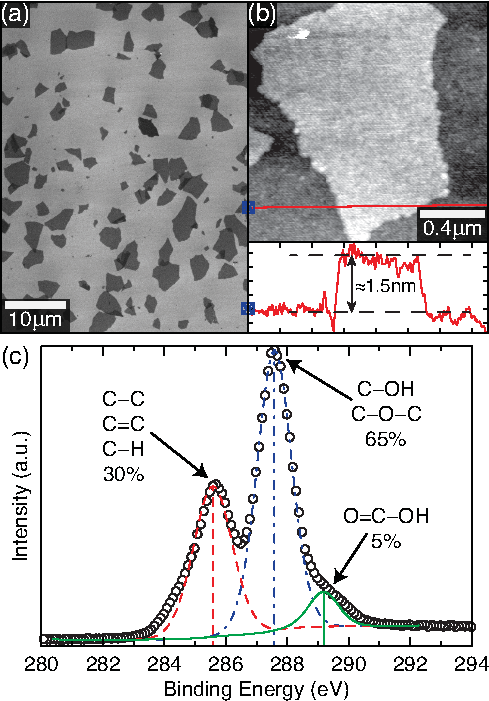
\includegraphics{paper1/Fig2.pdf}
  \caption{\textbf{Morphology and surface chemistry of GO flakes.} \textbf{(a)} SEM image of GO on Si wafer. \textbf{(b)} AFM image and line scan of the GO flakes. \textbf{(c)} XPS of GO flakes.}
  \label{fig2}
\end{figure}

\subsection{Morphology and Surface Chemistry of Graphene Oxide Nanoscrolls}
GONS produced by HF ultrasonic irradiation exhibit concentric geometries with a distinguishable number of outer-walls as displayed in Fig.~\ref{fig3}a \textit{e.g.}, six walls for the top-left GONS. This indicates that the GONS produced here are of high quality, similar to a recent report,\cite{Kim2014} as they are not assemblies of crumpled and/or folded GO layers. The resulting GONS were characterized by two distinct geometries: a constant outer diameter tube-like GONS (T-GONS); and a variable outer diameter cone-like GONS (C-GONS). The formation of T-GONS is a result of a constant scrolling speed and/or direction whereas surface inhomogeneities/defects may cause a variable speed/direction resulting in C-GONS formation.\cite{Hwang2014} SEM images illustrating the scrolling process that leads to the formation of both T-GONS and C-GONS structures (Fig.~\ref{figS1_AppB} and Fig.~\ref{figSa_AppB}) and TEM images that illustrate the hollow nature of the produced GONS (Fig.~\ref{figS2_AppB}) can be found in the Appendix B.

Narrow and wide T- and C-GONS structures are observed and characteristic diameters were quantified by SEM image analysis (Fig.~\ref{fig3}a). Narrow T-GONS structures are characterized by $d_{\mathrm{tube}} = 215 \pm 75$ nm, while narrow C-GONS structures exhibit a minimum diameter $d_{\mathrm{cone,min}} = 215 \pm 75$ nm and maximum diameter of $d_{\mathrm{cone,max}} = 1.65 \pm 0.39\ \mu$m. Wide GONS structures have $d_{\mathrm{tube}} = 1.80 \pm 0.27\ \mu$m for T-GONS and $d_{\mathrm{cone,min}} = 0.95 \pm 0.32\ \mu$m and $d_{\mathrm{cone,max}} = 1.84 \pm 0.33\ \mu$m for C-GONS. Note for narrow GONS $d_{\mathrm{tube}} \sim d_{\mathrm{cone,min}}$, and for wide GONS $d_{\mathrm{tube}} \sim d_{\mathrm{cone,max}}$. Size distribution histograms are displayed in Fig.~\ref{figS4_AppB} of the Appendix B.  The observed GONS diameters are related to the area of the parent GO flake and the inter-layer separation of the GONS walls. The GONS have an observed inter-layer separation on the order of $10-100$ nm,\cite{Fan2015} as can be seen in Fig.~\ref{fig3}a, which is much larger than the inter-layer separation of GNS and CNT ($\approx0.34$ nm).\cite{Zhang2010} Thus, the GONS inter-wall regions will be more accessible to atoms and molecules than GNS/CNT, providing utility for applications requiring readily accessible surface areas such as adsorptive and capacitive processes.
Another important factor that may contribute to variations in $d_{\mathrm{min}}$ is related to the extent of GO flake oxidation and surface chemistry, which in turn will affect the elastic modulus of GO\cite{Liu2012}
and weaken inter-layer $\pi-\pi$ interactions.\cite{Hwang2014} The GO and GONS structures were characterized via Raman spectroscopy and both display a D-band (A$_{1\mathrm{g}}$ symmetry) at $\approx1350$ cm$^{-1}$ representative of defects/disorder in the basal plane and a G-band (E$_{2\mathrm{g}}$ symmetry) at $\approx 1590$ cm$^{-1}$ that corresponds to the in-plane sp$^{2}$ bond stretching.\cite{Ferrari2000,Dresselhaus2010,Ferrari2013,Ferrari2006} The G-band full width half maximum (FWHM) of the GONS is larger than the FWHM of the G-band of pristine graphene and bulk graphite,\cite{Ferrari2006,Rao2011} \textit{i.e.} $\approx 20$ cm$^{-1}$,\cite{Casiraghi2007} as displayed in Fig.~\ref{fig3}b. To quantitatively analyze the relative defect density of the GO and GONS, the Raman spectra were fit ($\mathbb{R}^{2} > 0.99$) using single Lorentzian (D-band) and Breit-Wigner-Fano (G-band) distributions as displayed in Fig.~\ref{fig3}b.\cite{Mallet2014,Mallet2014a} The D- and G-band fits indicate that the FWHM of the D-band remains constant at $119 \pm 6$ cm$^{-1}$ after GONS formation, whereas the FWHM of the G-band increases from $64 \pm 3$ to $78 \pm 4$ cm$^{-1}$. The broader GONS G-band is due to scrolling effects on the basal plane breathing mode\cite{Xie2009} since the formation of a multi-layer morphology will increase elastic strain\cite{Roy2008,Gao2010} e.g., GONS or overlapped GO layers as displayed in Fig.~\ref{figS5_AppB}. The D/G intensity ratio ($I_{\mathrm{D}}/I_{\mathrm{G}}$) was 1.1 for both GO and GONS,\cite{Gao2010} and the D/G area ratio ($A_{\mathrm{D}}/A_{\mathrm{G}}$) decreased from $\approx 1.4$ for GO to $\approx 1.2$ for GONS suggesting that GONS formation is facilitated by GO with fewer oxygen functional groups, and more $\pi-\pi$ interactions.\cite{Hwang2014} The fitted G band peak position for the GONS is red-shifted by $\approx 10$ cm$^{-1}$ as compared to the original GO flakes, which is indicative of reduced disorder in nanocrystalline graphitic materials,\cite{Ferrari2000} in agreement with the decrease in $A_{\mathrm{D}}/A_{\mathrm{G}}$ from GO to GONS. The $\approx 15$ cm$^{-1}$ increase of the GONS G-band FWHM can be utilized to distinguish the GO and GONS using a spatially-dependent integration (50 nm resolution) of the G-band intensity (Fig.~\ref{fig3}c-right) where the GONS are of higher integrated intensity (compare to SEM; Fig.~\ref{fig3}c left) that originates from the broader G-band of GONS caused by the phenomena explained above.

\begin{figure}[t!]
  \centering
  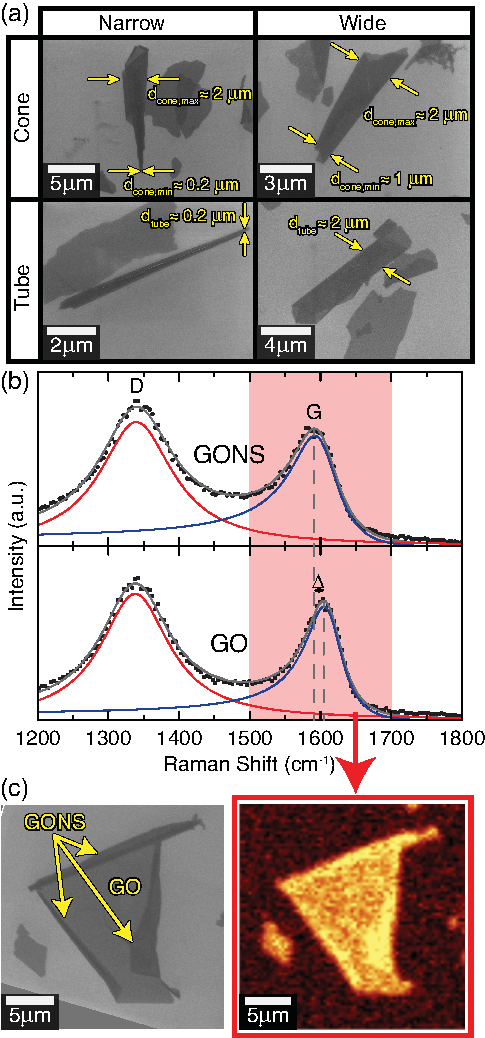
\includegraphics{paper1/Fig3.pdf}
  \caption{\textbf{Morphology and defect density of GONS.} \textbf{(a)} SEM displaying narrow and wide cone-like (C-GONS) and tube-like (T-GONS) that are characterized by their diameters ($d_{\mathrm{tube}}$) and ($d_{\mathrm{cone}}$). \textbf{(b)} Raman spectra of the D- and G-bands for GO and GONS. \textbf{(c)} SEM and spatial integration of G-band intensity of a partially-scrolled GO where scrolled regions are of greater intensity than the flat regions.}
  \label{fig3}
\end{figure}

\subsection{Effect of Ultrasonic Frequency on Dimensions}

The effect of ultrasound frequency (20 kHz LF vs. 390 kHz HF) and power density on the GO flake area ($A_{\mathrm{GO}}$) and GONS length ($L_{\mathrm{GONS}}$) as a function of the ultrasonic irradiation time ($t$) was evaluated as displayed in Fig.~\ref{fig4}. Calorimetry indicates that $\approx10^{3} - 10^{4}$ J mol$^{-1}$ is introduced to the GO solutions during the 1 hr ultrasonic treatments (see Methods section for calorimetry calculation), which is similar to the previously reported theoretical energy barrier for scrolling graphene.\cite{Braga2004,Patra2009} Since we can observe GONS formation at treatment times as short as 5 min where only $10^{2}$ J mol$^{-1}$ is introduced, the calorimetry suggests that the GONS scrolling process may occur at local `hot spots' generated by bubble cavitation.\cite{Suslick1986,Kotronarou1991} Calorimetry also indicates that both LF and HF ultrasonic irradiation transfer $\approx10$ W to the GO solution, thus observed differences in $A_{\mathrm{GO}}$ and $L_{\mathrm{GONS}}$ can be attributed to the difference in ultrasonic frequency.

For both ultrasonic frequencies, $A_{\mathrm{GO}}$ decreases over the 60 min irradiation time with the majority of the decrease occurring over the first $10-20$ min of irradiation from $A_{\mathrm{GO}}(t = 0) = 53 \pm 4\ \mu$m$^{2}$ to $A_{\mathrm{GO}}^{\mathrm{HF}}(t = 60) = 30 \pm 2\ \mu$m$^{2}$ and to $A_{\mathrm{GO}}^{\mathrm{LF}}(t = 60) = 7 \pm 0.7\ \mu$m$^{2}$. A similar decrease is observed for $L_{\mathrm{GONS}}$ as presented in Fig.~\ref{fig4}b, where the majority of the length decrease occurs over the first $20-30$ min from $L_{\mathrm{GONS}}^{\mathrm{HF}}(t = 5) = 11 \pm 1\ \mu$m to $L_{\mathrm{GONS}}^{\mathrm{HF}}(t = 60) = 7 \pm 0.8\ \mu$m and from $L_{\mathrm{GONS}}^{\mathrm{LF}}(t = 5) = 7 \pm 0.6\ \mu$m to $L_{\mathrm{GONS}}^{\mathrm{HF}}(t = 60) = 3 \pm 0.2\ \mu$m. For both cases, $A_{\mathrm{GO}}$ and $L_{\mathrm{GONS}}$ are relatively constant after the first 30 minutes of irradiation, a favorable time-window for industrial-scale processing. Note that $L_{\mathrm{GONS}}$ achieves a minimum after $A_{\mathrm{GO}}$ achieves a minimum and hat the final $A_{\mathrm{GO}}$ is roughly the same as the final $L_{\mathrm{GONS}}^{2}$ suggesting that the energy to scroll GO is less than the energy to cleave. Additional details pertaining to the GO and GONS dimensions can be found in the Appendix B. The $A_{\mathrm{GO}}$ and $L_{\mathrm{GONS}}$ results indicate that the LF ultrasonic irradiation is harsher than the HF treatment as expected. The cavitation energy released during transient adiabatic bubble collapse is proportional to $R_{\mathrm{max}}^{3}$ where $R_{\mathrm{max}}$ is the maximum bubble radius ($P$d$V$ energy release)\cite{Tinguely2012} and the 20 kHz LF treatment generates bubbles that are more than an order of magnitude larger than the bubbles formed by the 390 kHz HF treatment\cite{Brotchie2009,Merouani2013}, \textit{i.e.} $R_{\mathrm{max}} \propto 1/f$ where $f$ is the ultrasonic frequency, resulting in significantly stronger LF individual bubble cavitation phenomena.

\begin{figure}[t!]
  \centering
  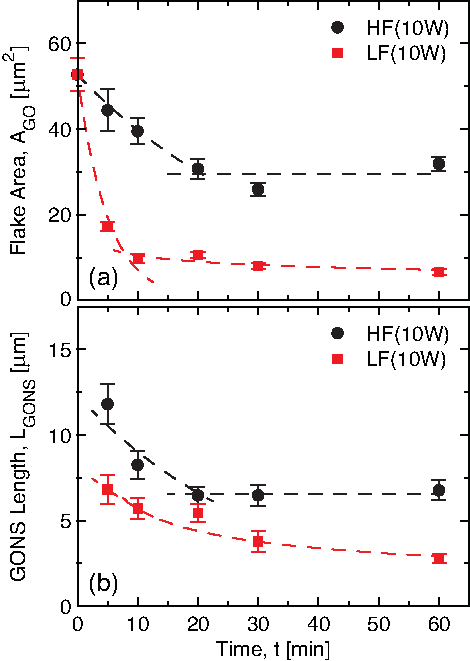
\includegraphics{paper1/Fig4.pdf}
  \caption{\textbf{Effect of ultrasonic frequency and irradiation time on GO and GONS dimensions.} \textbf{(a)} Plot of the GO area ($A_{\mathrm{GO}}$) for the low frequency (LF) and high frequency (HF) treatment at 10 W of calorimetric power as a function of the irradiation time $t$. \textbf{(b)} Plot of the GONS length ($L_{\mathrm{GONS}}$) as a function of $t$ for the two conditions. The fitting lines are based on eq~(\ref{eqn1}) and eq~(\ref{eqn2}).}
  \label{fig4}
\end{figure}
\subsection{Effect of Ultrasonic Power Density on Dimensions}
The effect of ultrasound calorimetric power density (HF 1, 10, \& 20 W; LF 10 \& 100 W) on the time-dependent $A_{\mathrm{GO}}$ and $L_{\mathrm{GONS}}$ is displayed in Fig.~\ref{fig5}. If the HF ultrasonic power is decreased to 1 W, then there is no significant change in $A_{\mathrm{GO}}$ with $t$, whereas increasing the HF ultrasonic power to 20 W (2-fold) decreases $A_{\mathrm{GO}}$ as compared to 10 W by 2-fold ($A_{\mathrm{GO}}^{\mathrm{HF(20\ \mathrm{W})}}(t = 60) = 15 \pm 1\ \mu$m$^{2}$). If the LF ultrasonic power is increased from 10 to 100 W, then the $A_{\mathrm{GO}}$ was decreased 3-fold($A_{\mathrm{GO}}^{\mathrm{LF(100\ \mathrm{W})}}(t = 60) = 2 \pm 0.2\ \mu$m$^{2}$). Similar trends were observed for $L_{\mathrm{GONS}}$ with regards to power and frequency as displayed in Fig.~\ref{fig5}b. For example, decreasing HF power to 1 W resulted in a negligible decrease of $L_{\mathrm{GONS}}$ with time suggesting there is not enough acoustic power for high-energy transient bubble cavitation and that stable cavitation may be enough to scroll GO. Increasing the HF ultrasonic power from 10 to 20 W results in a negligible change in $L_{\mathrm{GONS}}^{\mathrm{HF(20\ \mathrm{W})}}(t)$, in contrast to the 2-fold reduction in $A_{\mathrm{GO}}(t)$, again indicating the GONS are more difficult to cleave than GO. However, increasing the LF power to 100 W resulted in a 3-fold decrease, in $L_{\mathrm{GONS}}$ ($L_{\mathrm{GONS}}^{\mathrm{LF(100\ \mathrm{W})}}(t = 60) = 1 \pm 0.1\ \mu$m), similar to the decrease in $A_{\mathrm{GO}}$.

\begin{figure}[t!]
  \centering
  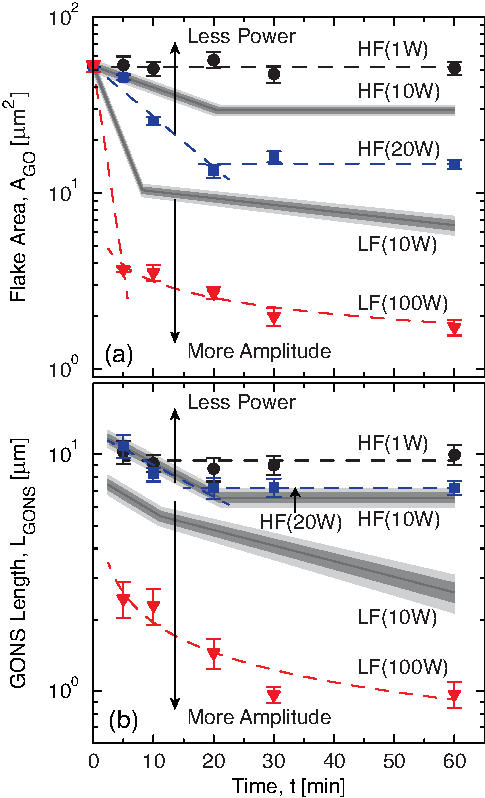
\includegraphics{Fig5.pdf}
  \caption{\textbf{Effect of ultrasonic power and frequency on GO area (a) and GONS length (b) as a function of time ($t$).} Black circles, blue squares, and red triangles refer to 1 W (HF), 10 W (HF) and 100 W (LF) irradiation power, respectively. Shaded grey trends represent experimental data from Fig.~\ref{fig4}. The fitting lines are based on eq~(\ref{eqn1}) and eq~(\ref{eqn2}).}
  \label{fig5}
\end{figure}

\begin{sidewaystable}
 \begin{center}
 \caption{Kinetic parameters for time-dependent GO and dimensional decrease. The critical time ($t_{\mathrm{crit}}$) is approximated via the intersection of the exponential scaling and power scaling. See eqn~(\ref{eqn1}) \& eqn~(\ref{eqn2}) for the functional forms.}
  \label{tbl1}
  \begin{tabular}{cc|ccccc|ccccc}
        \hline
        Process & Power & $A_{1}$ & $k_{\mathrm{GO}}$ & $A_{2}$ & $s_{1}$ & $t_{\mathrm{crit}}$ & $L_{1}$ & $k_{\mathrm{GONS}}$ & $L_{2}$ & $s_{2}$ & $t_{\mathrm{crit}}$ \\
         & [W] & [$\mu$m$^{2}$] & [min$^{-1}$] & [$\mu$m$^{2}$] & [] & [min] & [$\mu$m] & [min$^{-1}$] & [$\mu$m] & [] & [min] \\
        \hline
        HF(1 W) & $1.2 \pm 0.3$ & $52.8$ & $0$ & $52.8$ & $0$ & $> 60$ & $9.43$ & $0$ & $9.43$ & $0$ & $> 60$ \\
        HF(10 W) & $10.2 \pm 2.3$ & $52.8$ & $0.028$ & $29.6$ & $0$ & $20.7$ & $12.6$ & $0.031$ & $6.56$ & $0$ & $21.1$ \\
        HF(20 W) & $19.7 \pm 3.9$ & $52.8$ & $0.066$ & $14.7$ & $0$ & $19.4$ & $12.3$ & $0.031$ & $7.22$ & $0$ & $17.2$ \\
        \hline
        LF(10 W) & $10.2 \pm 2.3$ & $52.8$ & $0.199$ & $17.3$ & $0.213$ & $7.8$ & $8.13$ & $0.035$ & $13.5$ & $0.375$ & $8.7$ \\
        LF(100 W) & $99.9 \pm 13.2$ & $52.8$ & $0.533$ & $6.42$ & $0.309$ & $4.9$ & $-$ & $-$ & $5.13$ & $0.421$ & $\leq 5$ \\
        \hline
  \end{tabular}
 \end{center}
\end{sidewaystable}
Here, the kinetics of $A_{\mathrm{GO}}$ and $L_{\mathrm{GONS}}$ dimension decrease are quantitatively examined to gain insight into the physical mechanisms that mediate ultrasonic cleavage. The two predominant mechanisms are: I) GO flake and GONS cleavage at defect (oxygen) sites ($E_{\mathrm{A}} = 50 - 60$ mJ mol$^{-1}$)\cite{Chakarova2006,Chen2013a,Felts2015} that was previously modeled with exponential kinetics\cite{Kouroupis2014,Rider2014} and II) cavitation mediated scission that was previously modeled using power kinetics.\cite{Khan2010,Paton2014} Mechanisms I and II can be modeled by kinetic eqn~(\ref{eqn1}) \& eqn~(\ref{eqn2}), respectively:
\begin{equation}
    A_{\mathrm{GO}}(t) = \begin{cases} A_{1}(e^{-k_{\mathrm{GO}}t}), & t \leq t_{\mathrm{crit}} \\ A_{2}(t)^{-s_{1}}, & t \geq t_{\mathrm{crit}} \end{cases}
    \label{eqn1}
\end{equation}

\begin{equation}
    L_{\mathrm{GONS}}(t) = \begin{cases} L_{1}(e^{-k_{\mathrm{GONS}}t}), & t \leq t_{\mathrm{crit}} \\ L_{2}(t)^{-s_{2}}, & t \geq t_{\mathrm{crit}} \end{cases}
    \label{eqn2}
\end{equation}
where $A_{1}$ and $A_{2}$ are constants related to the area of the GO flakes, $L_{1}$ and $L_{2}$ are constants related to the GONS length, $k_{\mathrm{GO}}$ and $k_{\mathrm{GONS}}$ are kinetic rate constants for mechanism I, and $s_{1}$ and $s_{2}$ are power exponents for mechanism II. Note the two mechanisms are operating simultaneously; however, mechanism I, is just much faster than the mechanism II. Once all of the defect sites are cleaved, the cavitation-based cleavage dominates the kinetics. The competing GO/GONS cleavage mechanism is modeled using a critical irradiation time ($t_{\mathrm{crit}}$), which represents the transition time point from defect-based cleavage Mode I ($t \leq t_{\mathrm{crit}}$) to the cavitation-based mechanical cleavage Mode II ($t \geq t_{\mathrm{crit}}$). Due to the high temperature of the surface of the bubbles (\textit{e.g.} $600 - 800$ \textdegree C), \textit{in situ} thermal reduction may also occur concurrently with the cleavage governed by Mode I and Mode II. For example, after 5 min of ultrasonic irradiation (LF and HF) the C-C/C=C peaks increased (30 to $60-65\%$), the C-O peak decreased (45 to $20-25\%$) and the O=C-O peak slightly increased (5 to 15\%) in the C1s spectrum (Fig.~\ref{figS6_AppB}).

Since the HF process generates smaller less-energetic and more spherical bubbles than the LF process,\cite{Brotchie2009,Merouani2013} mechanical scission likely does not occur to a significant extent \textit{e.g.}, $s_{1}$ and $s_{2}$ for HF are negligible. The LF produces larger bubbles that undergo more energetic and non-spherical collapse of bubbles during sonication leading to the formation of microjets\cite{Xu2013,Han2014} that are known to cause scission in graphene and CNTs.\cite{Khan2010,Hennrich2007,Lucas2009,Pagani2012} The LF exponents $s_{1}$ and $s_{2}$ range from $0.21 \leq s_{1} \leq 0.31$ and $0.38 \leq s_{2} \leq 0.42$ (See Table~\ref{tbl1}). These values are in good agreement with the previously reported exponents of $\approx0.21 - 0.25$ for scission of micrometer-long CNTs ($s_{1}$ scission of GO flakes),\cite{Lucas2009,Pagani2012} and exponents of $\approx0.41 - 0.5$ for scission of short CNTs ($s_{2}$ scission of GONS).\cite{Hennrich2007,Pagani2012} $L_{1}$, $L_{2}$, $k_{\mathrm{GONS}}$, and $s_{2}$ for HF(10W) and HF(20 W) are nearly identical demonstrating that the HF treatment is not effective at producing short GONS, which may be desired during processing. These previously reported kinetic coefficients are valid irrespective of the solution volume used during the ultrasonic treatment, and are in good agreement with an LF(10W) treatment done using a smaller beaker and GO solution volume (see Fig.~\ref{figSb_AppB}in the Appendix B). Further work is required to elucidate the fundamental mechanism of Mode I and how $t_{\mathrm{crit}}$ can be controlled.
\section{Conclusions}
The synthesis of graphene oxide nanoscrolls with tunable dimensions was achieved via 20 kHz low frequency and 390 kHz high frequency solution processing techniques. Simultaneous fine-tuning of GO flake dimensions and surface chemistry was achieved in a industrial-scale time window. Electron microscopy indicates that the produced GONS exhibit well-defined tube or cone geometries with a finite number of walls. Raman spectroscopy indicates that defect concentration, decreases from the parent GO ($A_{\mathrm{D}}/A_{\mathrm{G}} \approx1.4$) to the resulting GONS ($A_{\mathrm{D}}/A_{\mathrm{G}} \approx1.2$) suggesting GO with lower defects have a lower scrolling activation energy. Two mechanisms are responsible for the ultrasonic reduction of the GO area and GONS length as a function of the irradiation time: cleavage at defect (oxygen) sites at short $t$ (exponential kinetics) and cavitation microjet mediated scission at long $t$ (power kinetics). XPS indicates that both LF and HF ultrasonication decreases GO C-O bonds and increases C-C bonds by at least 2-fold, likely due to in situ thermal reduction at the cavitating bubble-water interface. Further work via experiments, theory, and simulation is required to model the underlying physics that govern these two mechanisms, and the effect of parent GO dimensions and surface chemistry. An understanding of the underlying ultrasonic that determine the characteristics of the produced GO and GONS will allow tunable modification of the diameter and surface chemistry for a range of applications.
